\section{Experiments}
\label{sec:experiments}

\subsection{Experimental Setup}

We evaluate our approach on 3DSRBench~\cite{ma2025spatialreasoner}, a comprehensive benchmark for 3D spatial reasoning containing 11,686 questions across diverse spatial relationship categories. The benchmark covers distance estimation, directional reasoning, size comparison, and complex spatial queries requiring multi-step inference. All models use Qwen2.5-VL-7B-Instruct~\cite{bai2025qwen25vl} as the base architecture, fine-tuned with LoRA (rank 256) using the same hyperparameters for fair comparison.

View synthesis is performed using MVGenMaster, which generates video sequences depicting camera motion around the scene. We extract the final frame corresponding to the target rotation angle. For the full benchmark, we pre-generate $10^\circ$ rotated views for all 3,587 unique images, ensuring consistent view quality across evaluation runs.

\subsection{Quantitative Analysis}

Table~\ref{tab:main-results} and Figure~\ref{fig:accuracy-comparison} present the main experimental results comparing our multi-view approach against baseline methods.

\begin{table}[ht]
\centering
\begin{tabular}{lc}
\toprule
\textbf{Model} & \textbf{Accuracy (\%)} \\
\midrule
\multicolumn{2}{l}{\textit{Proprietary Models}} \\
GPT-4o~\cite{openai2024gpt4o} & 44.2 \\
Gemini 2.0~\cite{google2024gemini} & 51.1 \\
Qwen2.5-VL-Max~\cite{bai2025qwen25vl} & 52.0 \\
\midrule
\multicolumn{2}{l}{\textit{Open-Source Models}} \\
Qwen2.5-VL-7B & 48.3 \\
SpatialReasoner-SFT~\cite{ma2025spatialreasoner} & 58.3 \\
SpatialReasoner~\cite{ma2025spatialreasoner} & 60.3 \\
\midrule
\multicolumn{2}{l}{\textit{Our Approach}} \\
+ SFT (reproduced) & 58.0 \\
+ SFT + Mixed Aug & 60.2 \\
+ MVGen Multi-View & 60.1 \\
\bottomrule
\end{tabular}
\caption{Accuracy on 3DSRBench. Results for proprietary and SpatialReasoner models are from~\cite{ma2025spatialreasoner}. Our multi-view approach achieves comparable performance to SpatialReasoner while using a different methodology based on synthesized view pairs.}
\label{tab:main-results}
\end{table}

\begin{figure}[ht]
\centering
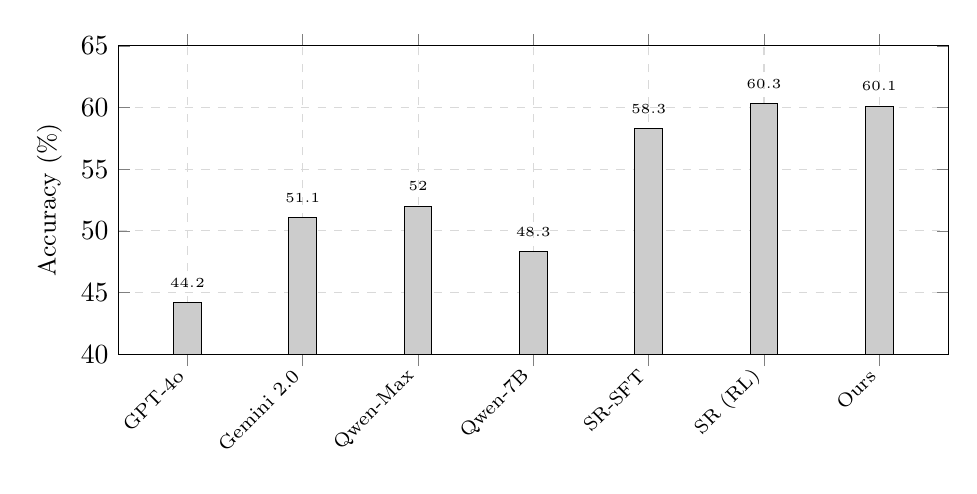
\begin{tikzpicture}
\begin{axis}[
    ybar,
    width=\columnwidth,
    height=5.5cm,
    ylabel={Accuracy (\%)},
    ylabel style={font=\small},
    ymin=40,
    ymax=65,
    ytick={40,45,50,55,60,65},
    xtick=data,
    symbolic x coords={GPT-4o, Gemini 2.0, Qwen-Max, Qwen-7B, SR-SFT, SR (RL), Ours},
    x tick label style={rotate=45, anchor=east, font=\scriptsize},
    bar width=10pt,
    nodes near coords,
    nodes near coords style={font=\tiny},
    every node near coord/.append style={yshift=2pt},
    enlarge x limits=0.1,
    grid=major,
    grid style={dashed, gray!30},
]
\addplot[fill=gray!40] coordinates {(GPT-4o, 44.2) (Gemini 2.0, 51.1) (Qwen-Max, 52.0) (Qwen-7B, 48.3) (SR-SFT, 58.3) (SR (RL), 60.3) (Ours, 60.1)};
\end{axis}
\end{tikzpicture}
\caption{Comparison on 3DSRBench. Our multi-view approach (Ours) achieves 60.1\% accuracy, comparable to SpatialReasoner with reinforcement learning (SR-RL, 60.3\%) while using a different methodology based on geometric consistency across synthesized views.}
\label{fig:accuracy-comparison}
\end{figure}

Among proprietary models, Gemini 2.0 achieves 51.1\% and Qwen2.5-VL-Max reaches 52.0\%, while GPT-4o shows lower performance at 44.2\%. SpatialReasoner~\cite{ma2025spatialreasoner} establishes the current state-of-the-art at 60.3\% through a combination of chain-of-thought supervision and reinforcement learning.

Our reproduced SFT baseline achieves 58.0\%, consistent with the reported SpatialReasoner-SFT result of 58.3\%. Adding mixed augmentation---horizontal flipping and color jittering applied to both images and corresponding spatial coordinates in the chain-of-thought annotations---further improves performance to 60.2\%.

The multi-view approach using MVGenMaster-synthesized views achieves 60.1\% accuracy when both training and inference utilize dual-view inputs. This result is comparable to both our mixed augmentation baseline and the full SpatialReasoner model, while employing a fundamentally different methodology. Rather than relying on reinforcement learning for improved reasoning, our approach leverages geometric consistency across synthesized viewpoints. The comparable performance suggests that explicit multi-view reasoning offers a viable alternative to RL-based refinement, though the additional computational cost of view synthesis should be considered in practical deployment.

\subsection{Qualitative Analysis}

Multi-view inference can provide advantages for spatially ambiguous scenarios, though systematic analysis of per-category improvements remains for future work. We discuss several potential cases where dual-view input may help resolve single-view ambiguities.

Single-view spatial reasoning struggles with depth ordering when objects lack strong monocular cues. Two coffee cups at similar image positions may have ambiguous front-back relationships from one viewpoint, but the rotated view reveals parallax displacement where the closer cup shifts more in the image plane, providing depth ordering information. Similarly, partial occlusions create spatial uncertainty that rotated views can help resolve; when one object partially obscures another, a different viewpoint often reveals previously hidden portions, enabling more accurate spatial relationship estimation. Objects of unknown size present another classic ambiguity, as a small nearby object and a large distant object may appear identical in single views. View synthesis provides parallax cues that can distinguish these cases, since nearby objects exhibit larger apparent motion under camera rotation.

The approach also shows limitations in certain scenarios. Complex scenes with numerous overlapping objects challenge the view synthesis model, occasionally producing inconsistent multi-view pairs. Additionally, scenes with planar geometry perpendicular to the rotation axis yield minimal parallax, reducing the benefit of dual-view input. These failure cases suggest directions for future improvement in view synthesis and adaptive rotation strategy selection.

% \begin{figure}[t]
% \centering
% \includegraphics[width=\columnwidth]{figures/qualitative.pdf}
% \caption{Qualitative examples showing multi-view disambiguation. Left: original view. Middle: synthesized rotated view. Right: model reasoning process utilizing both views for spatial inference.}
% \label{fig:qualitative}
% \end{figure}
